\documentclass[12pt,a4paper,sans]{moderncv}
    \moderncvstyle{banking}
    \moderncvcolor{black}
    \nopagenumbers{}

    \usepackage[utf8]{inputenc}
    \usepackage[top=0.8cm, bottom=0.8cm, left=1cm, right=1cm]{geometry}
    \usepackage{ragged2e}
    \usepackage{multicol}
    \usepackage{enumitem}
    \usepackage{amssymb}
    \usepackage{fontawesome5}
    \usepackage{xcolor}
    \usepackage{hyperref}
    \hypersetup{colorlinks=true, urlcolor=blue}

    % Custom cventry
    \newcommand*{\customcventry}[7][.10em]{%
    \begin{tabular}{@{}l}
        {\bfseries #4} \\
        {\itshape #3}
    \end{tabular}
    \hfill
    \begin{tabular}{l@{}}
        {\bfseries #5} \\
        {\itshape #2}
    \end{tabular}
    \ifx&#7&%
    \else{\\
    \begin{minipage}{\maincolumnwidth}%
        \footnotesize#7%
    \end{minipage}}\fi%
    \par\addvspace{#1}
    }

    \begin{document}

    % En-tête : image à gauche, texte à droite
    \begin{minipage}{0.15\textwidth}
        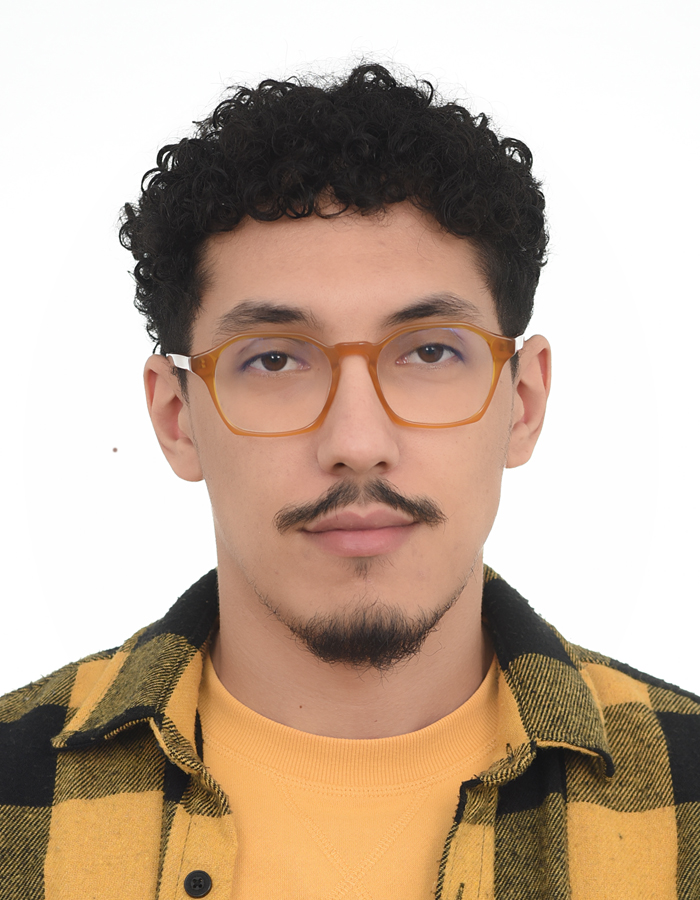
\includegraphics[width=\linewidth]{images/ahmed.jpg}
    \end{minipage}
    \hfill
    \begin{minipage}{0.82\textwidth}
        \centering
        {\fontsize{25}{28}\selectfont\textbf{Ahmed MAKROUM}}\\[0.3em]
        {\fontsize{15}{18}\selectfont Ingénieur Data et Développeur Full-Stack Web/Mobile} \\[0.4em]
        {\fontsize{11}{13}\selectfont
            \faMobile\enspace +212 6 64 71 52 19 \quad
            \faEnvelope\enspace ahmedmakroum3@gmail.com \quad
            \faHome\enspace Casablanca, Maroc \\[0.3em]
            \faLinkedin\enspace \href{https://www.linkedin.com/in/ahmed-makroum/}{in/ahmedmakroum} \quad
            \faGithub\enspace \href{https://github.com/ahmedmakroum}{github.com/ahmedmakroum} \quad
            \faGlobe\enspace \href{https://ahmedmakroum.github.io/AhmedMakroumPortfolio/}{makroum.me}
        }
    \end{minipage}

    \vspace{0,5em}

        % PROFIL
    \section{Profil}
    \justifying
    Ingénieur en informatique et réseaux (MIAGE : Méthodes Informatiques Appliquées à la Gestion des Entreprises) avec une solide expérience en ingénierie logicielle, data engineering et développement full-stack. Compétent dans la création de pipelines de données robustes, le développement d'applications web/mobile évolutives et l'utilisation des technologies cloud et open source. Reconnu pour son adaptabilité, son esprit d'équipe et sa passion pour l'apprentissage continu.

    % EXPÉRIENCE
    \section{Expérience}
    \customcventry{03/2025 ‐ Présent}{\href{https://www.allianz.ma}{Allianz Maroc}}{Ingénieur Data}{}{}{
    \begin{itemize}[leftmargin=0.5cm, itemsep=0pt, topsep=0pt]
    \item Conception et déploiement de pipelines de données de bout en bout avec NiFi et Spark pour extraire, nettoyer et charger les données des systèmes internes d'assurance.
    \item Consolidation de sources fragmentées dans un entrepôt PostgreSQL, permettant des rapports unifiés et cohérents.
    \item Mise en place de tableaux de bord temps réel avec Metabase, améliorant l'accès aux données pour les utilisateurs métier.
    \item Développement et maintenance d'une application web pour la gestion et le suivi des paiements santé d'Allianz vers les prestataires externes, avec Spring Boot et Next.js.
    \end{itemize}}
    \customcventry{06/2024 ‐ 08/2024}{\href{https://boti.education/}{BOTI School}}{Ingénieur Data}{}{}{
    \begin{itemize}[leftmargin=0.8cm, itemsep=0pt, topsep=0pt]
    \item Développement d'un pipeline ETL évolutif avec Apache Beam sur Google Cloud pour traiter les logs d'activité d'apprentissage.
    \item Transformation des données brutes en jeux de données structurés, permettant une meilleure compréhension du comportement utilisateur.
    \item Livraison de rapports automatisés via des tableaux de bord Looker pour la direction.
    \end{itemize}}

    \customcventry{06/2023 ‐ 08/2023}{\href{https://6solutions.com/}{6solutions}}{Développeur Web et Mobile}{}{}{
    \begin{itemize}[leftmargin=0.8cm, itemsep=0pt, topsep=0pt]
    \item Développement d'une plateforme de consulting multi-services (juridique, médical, financier).
    \item Réalisation du frontend web avec Angular et du backend avec Spring Boot.
    \item Conception et déploiement de l'application mobile sous Flutter, améliorant l'accessibilité pour les utilisateurs finaux.
    \end{itemize}}

    \customcventry{07/2022 ‐ 08/2022}{\href{https://estatmar.ma/}{Finso}}{Développeur Jeux Vidéo}{}{}{
    \begin{itemize}[leftmargin=0.8cm, itemsep=0pt, topsep=0pt]
    \item Conception et développement d'un jeu éducatif mobile pour enfants sous Unity.
    \item Création d'une expérience interactive axée sur l'apprentissage par le jeu.
    \item Renforcement de l'UX et de la logique d'animation dans un contexte de publication réelle.
    \end{itemize}}

        % PROJETS
    \section{Projets}
    \vspace{0.5em}
    \begin{itemize}[leftmargin=0.7cm, itemsep=2pt, topsep=2pt]
        \item \textbf{Plateforme de Consulting Marocaine} (\href{https://6solutions.ma/}{6solutions}) – Pilotage du développement d'une plateforme full-stack reliant les utilisateurs à des experts juridiques, médicaux et financiers. Réalisée avec React, Flutter, Node.js et PostgreSQL. \textit{Impact : 1000+ consultations en 3 mois.}
        \item \textbf{Pipeline de Données Assurance} (\href{https://www.allianz.ma/}{Allianz Maroc}) – Conception et déploiement de pipelines ETL robustes avec Apache NiFi et Spark pour unifier et exposer les données d'assurance à des fins d'analyse et de reporting.
        \item \textbf{Jeu Éducatif pour Enfants} (\href{https://finso.ma/}{Finso}) – Développement d'un jeu mobile Unity pour initier les enfants aux mathématiques et à la logique par le jeu. \textit{Résultat : 500+ téléchargements le premier mois.}
        \item \textbf{ETL Cloud pour Données d'Apprentissage} (\href{https://www.botischool.com/}{BOTI School}) – Construction d'un pipeline ETL évolutif sur Google Cloud avec Apache Beam, transformation et stockage de données éducatives à grande échelle.
        \item \textbf{Portfolio Personnel} (\href{https://ahmedmakroum.github.io/AhmedMakroumPortfolio/}{makroum.me}) – Création et déploiement d'un portfolio moderne et responsive pour présenter projets et compétences. Réalisé avec Next.js et hébergé sur GitHub Pages.
    \end{itemize}

    % FORMATION
    \vspace{-3mm}
    \section{Formation}

\customcventry
    {2020 -- 2025}
    {\href{https://emsi.ma}{\textbf{EMSI – École Marocaine des Sciences de l’Ingénieur}}}
    {Master MIAGE en Ingénierie Logicielle et Réseaux\\(Méthodes Informatiques Appliquées à la Gestion des Entreprises)}
    {}{}{}

    \customcventry
        {Juil. 2024 ‐ Sep. 2024}
        {\href{https://www.alxafrica.com}{\textbf{ALX Academy}}}
        {Diplôme d'Associé en Intelligence Artificielle et Prompt Engineering}
        {}{}{
        \begin{itemize}[leftmargin=0.5cm, itemsep=0pt, topsep=0pt]
            \item ALX AiCE – Fondamentaux de Carrière en IA
        \end{itemize}
        }

        % CERTIFICATIONS
        \section{Certifications}
        \textit{Tous les certificats ci-dessous ont été obtenus via Coursera.}
        \begin{itemize}[leftmargin=0.7cm, itemsep=2pt, topsep=2pt]
            \item \textbf{\href{https://www.coursera.org/account/accomplishments/verify/G178XXP17WQA}{Machine Learning with Python}} (IBM)
            \item \textbf{\href{https://www.coursera.org/account/accomplishments/records/M5RKGX36BAVA}{IBM Data Engineering}} (IBM)
            \item \textbf{\href{https://www.coursera.org/account/accomplishments/verify/2QK7QK7QK7QK}{Google Business Intelligence}} (Google)
            \item \textbf{\href{https://google.com}{Développement de Microservices Java évolutifs avec Spring Boot et Spring Cloud}} (Google Cloud)
            \item \textbf{\href{https://www.coursera.org/account/accomplishments/verify/EK5SJM3YM7PX}{Introduction au Big Data avec Spark et Hadoop}} (IBM)
            \item \textbf{\href{https://www.coursera.org/account/accomplishments/specialization/B4RCUAYCUG49}{Python for Everybody Specialization}} (Université du Michigan)
        \end{itemize}
    % COMPÉTENCES
    \vspace{-0,5em}
    \section{Compétences}
    \begin{itemize}[leftmargin=0.5cm, itemsep=0pt, topsep=0pt]
    \item \textbf{Data Engineering :} ETL, Apache NiFi, Spark, Beam, PostgreSQL, GCP
    \item \textbf{Programmation :} C, Python (pandas, FastAPI), SQL (PostgreSQL, MySQL), Java, TypeScript, 
    \item \textbf{Développement Web/Mobile :} React, Next.js, Flutter, Spring boot, APIs REST
    \item \textbf{DevOps :} Agilité, Docker, Kubernetes, Git, GitLab CI/CD, Linux
    \item \textbf{Visualisation :} Metabase, Superset, Power BI
    \item \textbf{Soft Skills :} Travail d'équipe, Communication, Adaptation, Résolution de problèmes
    \end{itemize}

    % EXTRASCOLAIRE
    \section{Activités Extrascolaires}
    Gestion de la logistique d'événements gaming et des relations sponsors pour le club F&G EMSI. Renforcement des partenariats, augmentation de la visibilité et amélioration des compétences en communication et négociation.

    % LANGUES
    \section{Langues}
    \begin{multicols}{2}
    \begin{itemize}[leftmargin=0.7cm, itemsep=2pt, topsep=2pt]
        \item \textbf{Anglais} – Courant
        \item \textbf{Français} – Courant
        \item \textbf{Arabe} – Langue maternelle
        \item \textbf{Espagnol} – Notions
    \end{itemize}
    \end{multicols}

% PIED DE PAGE
\vspace{1em}
\begin{center}
    {\footnotesize\color{gray}
    Pour en savoir plus sur mes projets et compétences, n'hésitez pas à consulter mon~
    \faLinkedin~\href{https://www.linkedin.com/in/ahmed-makroum/}{LinkedIn}~ou~\faGithub~\href{https://github.com/ahmedmakroum}{GitHub}.}
\end{center}

\end{document}
